\begin{figure*}
    \centering
    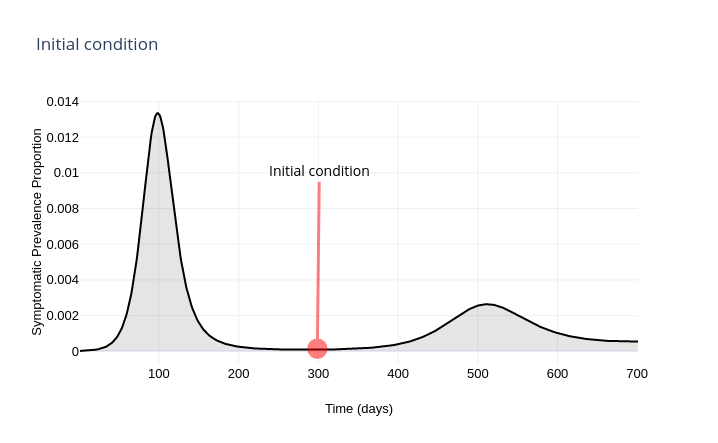
\includegraphics[scale=0.5, keepaspectratio]{figs/InitialCondition}
    \caption[Initial condition]{
        Initial condition scheme. We assume a positive
        prevelance. Forreference, at the date of write this manuscript,
        prevalence in CDMX is
        around \SI{16000}{cases}, see
        \href{https://plotly.com/~sauld/36/}{https://plotly.com/~sauld/36/}
        to display a electronic viewer.}
        \label{fig:initialcondition}
\end{figure*}

\begin{figure*}[tbh]
    \centering
    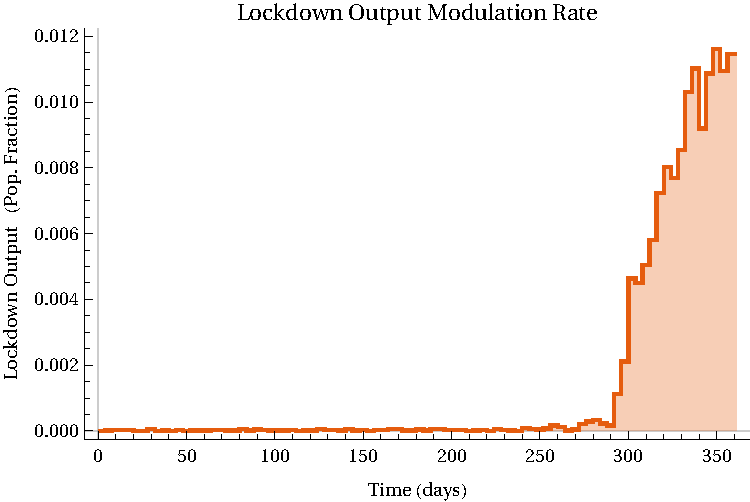
\includegraphics[width=0.7\linewidth]{figs/lockdown_control_signal}
    \caption[Lockdown modulation signal.]{Lockdown modulation signal.
    \href{https://plotly.com/~AdrianSalcedo/56/}
    {https://plotly.com/~AdrianSalcedo/56/}
            to display a electronic viewer.}
    \label{fig:lockdowncontrolsignal}
\end{figure*}

\begin{figure}
    \centering
    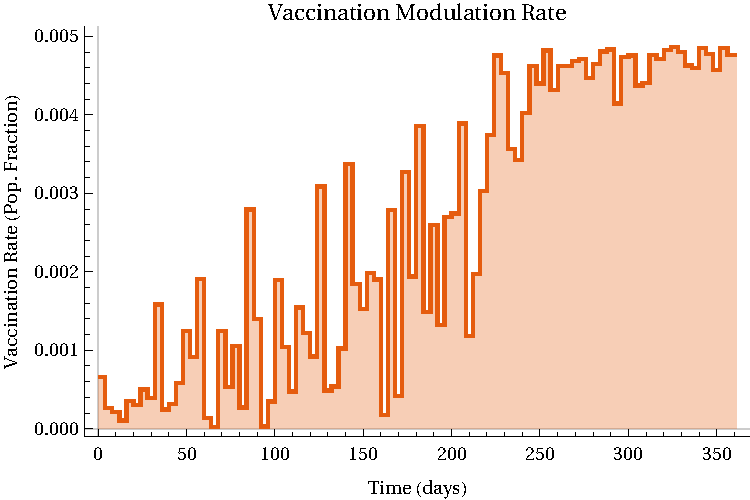
\includegraphics[width=0.7\linewidth]{figs/Vaccination_control_signal}
    \caption[Vaccination rate modulation.]{Vaccination rate modulation.
    \href{https://plotly.com/~AdrianSalcedo/58/}
    {https://plotly.com/~AdrianSalcedo/58/}}
    \label{fig:vaccinationcontrolsignal}
\end{figure}

\begin{figure}[tbh]
    \centering
    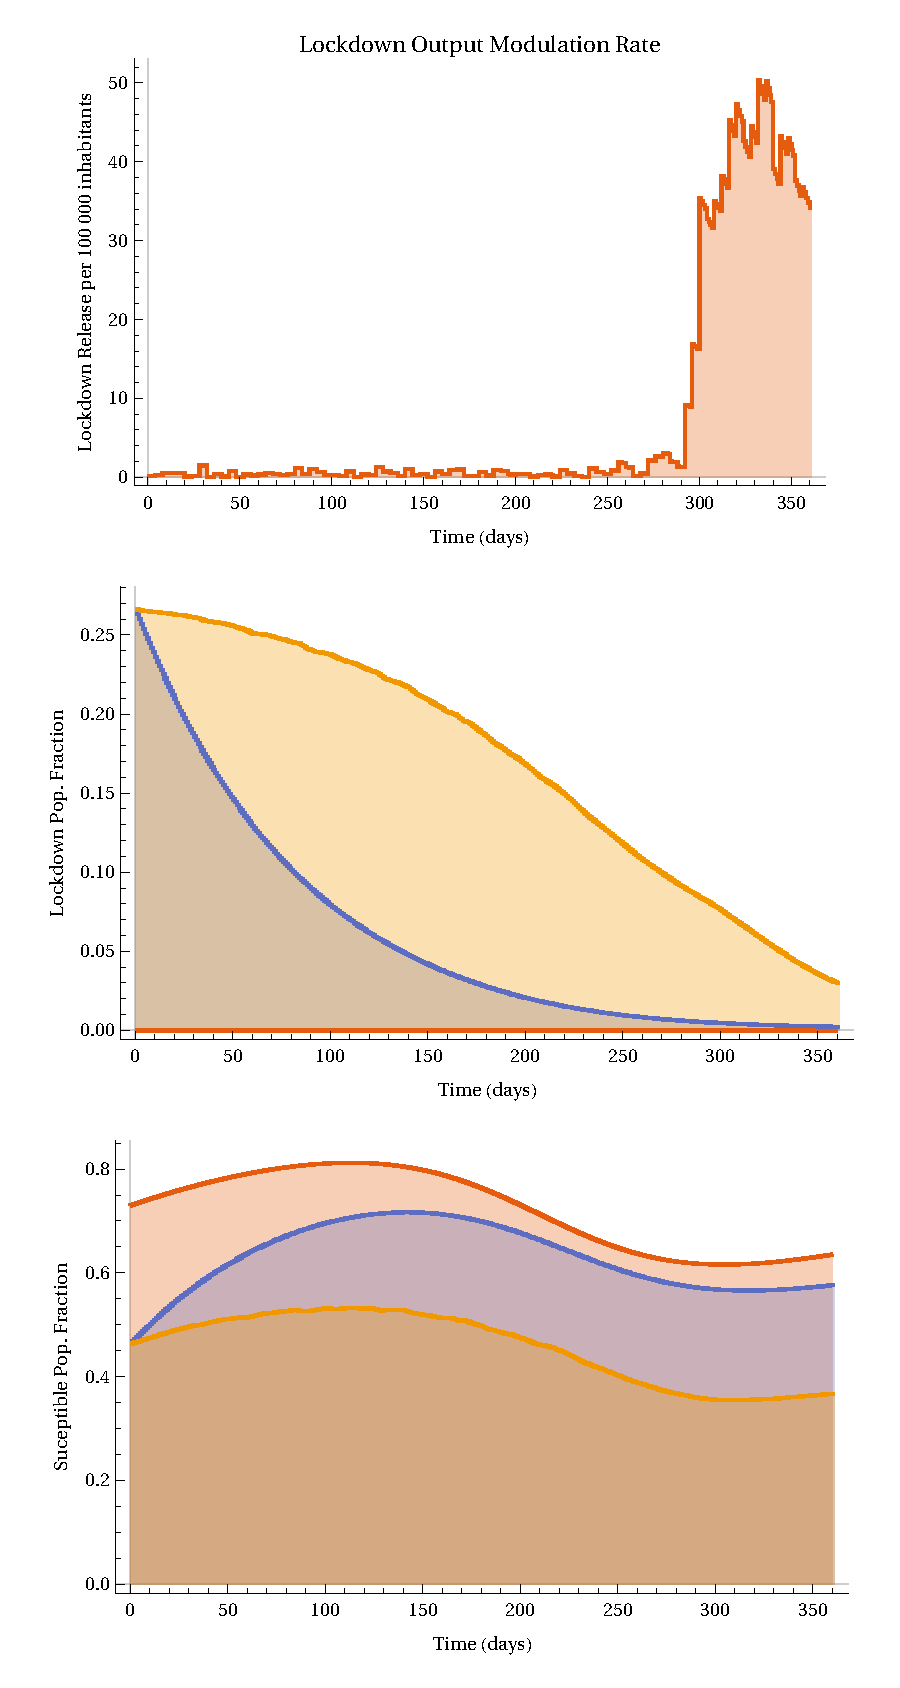
\includegraphics[scale=0.65, keepaspectratio]{figs/LockdownEffect}
    \caption{Modulation lock down release.
    \href{https://plotly.com/~AdrianSalcedo/60/}
    {https://plotly.com/~AdrianSalcedo/60/}}
    \label{fig:lockdowneffect}
\end{figure}

\begin{figure*}[tbh]
    \centering
    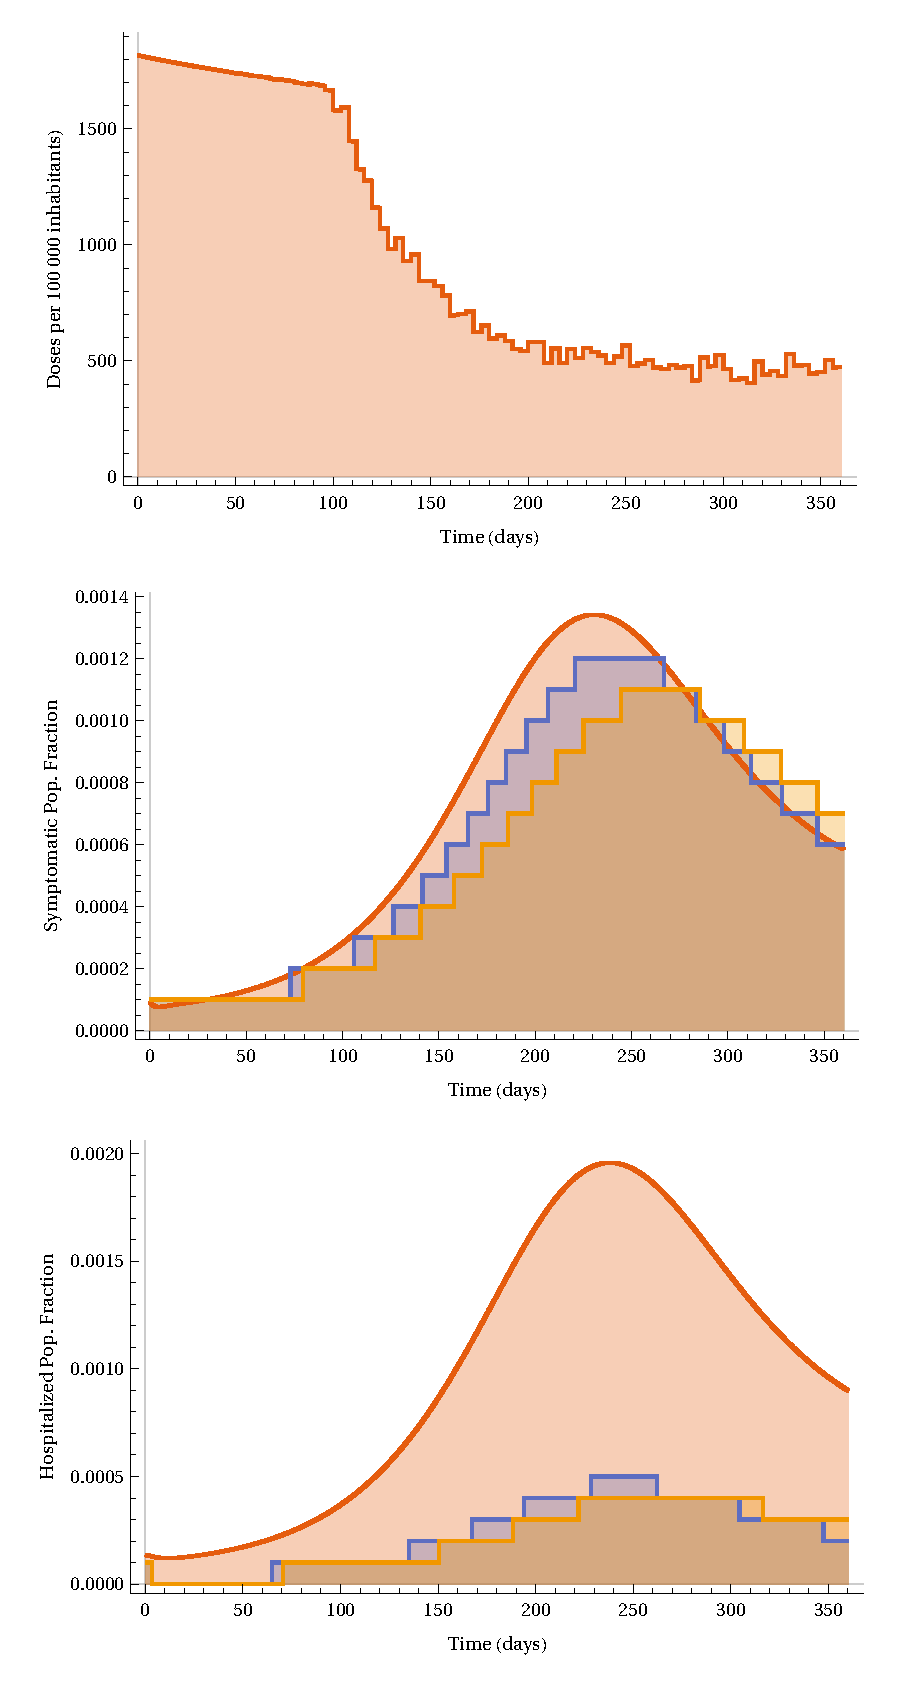
\includegraphics[scale=0.65, keepaspectratio]{figs/VaccinationEffect}
    \caption{Symptomatic Prevalence and Hozpitalization.
        \href{https://plotly.com/~AdrianSalcedo/61/}
        {https://plotly.com/~AdrianSalcedo/61/}}
    \label{fig:vaccinationeffect}
\end{figure*}
